\usepackage{hyperref}
\usepackage{graphicx}
\usepackage{listings}
\usepackage{textcomp}
\usepackage{fancyvrb}

\title{Ethics in Software Development: Time Traveler Edition}
\subtitle{Back...from the future}
\author{Moshe Zadka -- https://cobordism.com}
\date{2019}

\begin{document}
\begin{titlepage}
\maketitle
\end{titlepage}

\frame{\titlepage}

\begin{frame}[fragile]
\frametitle{Who am I}

\begin{itemize}
\item Born: July 10th, 2258
\item Certified Software Developer (passed exams Jan 22nd, 2287)
\item No formal higher education
\end{itemize}

\end{frame}

I have to let you all in on a little secret.
I was born in the future.
2258, to be precise.
Until I travelled back in time,
I was working as a certified software developer ever since
I passed my exams in 2287.

I don't want to go into the details of my time travel.
I want to talk about the differences in software development.
I want to talk about software developer ethics.
A code of ethics.
But what is a code of ethics?


\begin{frame}[fragile]
\frametitle{Ethic codes are trolleys}

\begin{figure}
\includegraphics[scale=0.25]{trolley}
\end{figure}

\end{frame}

Ultimately, a code of ethics consists of
"solutions"
to trolley problems:
a case where,
regardless of what we do,
some damage will be done.
A code of ethics tells us who to damage.
In the most of extreme of cases,
a code of ethics tells us who to kill.

So why do we want a code of ethics?
Why do we want to kill?
It is because in some professions,
you are going to be responsible for the life of people.
This responsibility for life is part of what you get
when you choose the profession.
This is something even you 21st century folks know:
some professions have accepted that part of their responsibilities
is making life and death decisions.

\begin{frame}[fragile]
\frametitle{Ethics in 21st century: civil engineers}

\begin{itemize}
\item Example: Act as faithful agent\pause
\item Example: Issue true statement\pause
\item Example: Service with competence
\end{itemize}

\end{frame}

Close to software developers,
civil engineers is also a profession where a lot of technical knowledge
and understanding of abstract principles is used to create
things people use every day.
Since they have been building things since the dawn of time,
and occasionally those collapse killing thousands,
civil engineers had to already think about what their ethics should look like.

\begin{frame}[fragile]
\frametitle{Ethics in 21st century: lawyers}

\begin{itemize}
\item Example: Confidentiality of information\pause
\item Example: Competence\pause
\item Example: No counsel to criminal actions
\end{itemize}

\end{frame}

Lawyers,
as welll,
have their code of ethics.
Part of their job is dealing with people who broke the law,
or possibly broke the law,
or who plan to have very interesting relationships with the law.
Regardless of whether the law is just or not,
a lawyer is not allowed to give advice to violate the law.
Regardless of how bad the secrets confided in them,
a lawyer cannot divulge them.

\begin{frame}[fragile]
\frametitle{Ethics in 21st century: doctors}

\begin{itemize}
\item Example: Responsibility to patient is paramount\pause
\item Example: Commitment to medical education\pause
\item Example: Report physicians engaging in fraud
\end{itemize}

\end{frame}

Another profession who can see their responsibility
for life and death,
since they deal,
often,
with bodies that are near death,
is doctors.
They have their own unique code of ethics,
that is applicable for their constraints.

However,
in the 21st century,
we have no widely accepted code of ethics.
The ACM has a code that has none of the rigor
that the other codes have,
and with none of the training that back them.
Of course,
the other thing the ACM code lacks is enforcement.
Doctors who violate ethics cannot practice medicine.
Lawyers cannot practice law.
There are no consequences for software developers.


\begin{frame}[fragile]
\frametitle{The Incident}

\begin{figure}
\includegraphics[scale=0.1]{volcano}
\end{figure}

\end{frame}

This,
in part,
is what led to the incident.
We do not like to talk about the incident.
I am not going to talk about it.
I'll just mention,
it was bad.
Really bad.
And there was no doubt that this was a direct cause
of software development being completely unregulated.

\begin{frame}[fragile]
\frametitle{The Incident: Causes}

\begin{figure}
\includegraphics[scale=0.5]{match}
\end{figure}

\end{frame}

There was a lot of public conversation about what led to the incident.
The first thing was that people realized that nobody is ever accountable
for software.
Everything comes with broad liability disclaimers.
Moreover,
nobody feels accountable for the final result.
Senior management off-loads to product managers,
product managers off-load to developers,
and they in turn off-load back to product managers,
or sometimes to QA.
Nobody feels responsible.
Nobody is in charge of managing user expectations,
and making sure they align with what the software does.
Most programmers work on one small part of the project,
and often have no visibility into what the project as a whole is supposed to do.
They often do not even know how this is intended to make money.

\begin{frame}[fragile]
\frametitle{The Incident: Consequences}

\begin{figure}
\includegraphics[scale=0.5]{fire}
\end{figure}

\end{frame}

What happened?
Trillions of dollars were lost,
either directly or as a result of 
something breaking.
People died.
Business went bankrupt.
It was pretty bad.
In 21st century term,
it was worse than 2008 financial crisis bad.
More like...world-war level of bad.

\begin{frame}[fragile]
\frametitle{The Incident: Aftermath}

\begin{figure}
\includegraphics[scale=0.5]{redtape}
\end{figure}

\end{frame}

In the aftermath of the incident,
finally,
the political will to internationally regulate software existed.
We went back to the basics.
What would make software fit to be used?
Who is allowed to write software that people will use?
How do we ensure that?

\begin{frame}[fragile]
\frametitle{23rd century}

It took a while...

\end{frame}

Figuring an entire regulatory structure for an existing industry took a while.
Imagine if driving regulation started a couple of hundred years after
cars were invented.
We had to figure out how to enact the regulation in a way that would
allow the software industry to adapt.
It probably would not have worked,
but the incident was so bad,
that whenever political will faltered,
someone would remind people how bad it can get.

Treaties were made.
Laws were confirmed.
We finally had a regulatory regime that allowed software to be safe for people.

\begin{frame}[fragile]
\frametitle{OS Updates}

\begin{itemize}
\item Signed
\item Mandatory
\end{itemize}

\end{frame}

We started with the basics:
what the operating system that runs on devices is supposed to look like.
OS updates were signed and mandatory.
A non-updated device would be disfunctional until it could get updated.
Device vendors had to commit to sending critical and security updates
for the lifetime of the device.

In particular,
for devices that were to be used for real work,
the OS and device maker were considered the same entity.
While the device maker could outsource the development of the OS,
they had final responsibility.

\begin{frame}[fragile]
\frametitle{Application stores}


\begin{figure}
\includegraphics{google_badge}
\end{figure}
\begin{figure}
\includegraphics[scale=0.15]{microsoft_badge}
\end{figure}


\end{frame}

However,
a device maker was explicitly barred from making decisions
as to what software is allowed to run on the device.
App stores would do that.
Specific rules for competitions between app stores were enacted.
A device maker
*could*
pre-load any app store,
but had to give a way for a user to add
*any*
licensed app store that supported the device.

Licensing an app store is non-trivial.
Among other things,
an app store has to have significant financial backing.
Since it is ultimately responsible for rogue apps,
it has to be able to pay out in case of a problem.
All big companies run an app store:
I will not give names,
since things have changed.

Translated to the 21st century,
every big company has an app store:
Google, Microsoft, Apple, Samsung,
Facebook, Disney and more.
There are about twenty "popular" app stores,
plus some niche stores.
Some stores specialize in devices from one company.
Some stores specialize in "ratings":
you can know that if an app is rated "G",
it really is safe for kids.

Some stores specialize in the exact opposite:
since most stores do not allow porn or porn-centric apps,
there is a market for porn-first app stores,
which explicitly allow for those apps.

Finally,
there is no difference between an "app store"
and a "certificate authority".
All apps use the 23rd century equivalent of TLS to connect to servers
when they do.
Apps will verify that the certificate authority of the server
is store they were installed through.
For general browsing,
installing a store is the same as installing a certificate authority,
and will allow connecting to web sites that were signed by this
authority.

In some sense,
it does not matter to the store which part of the app runs on the device,
and which part runs on the server:
the store certifies the whole thing is both fit for use,
and complies with whatever guidelines the store has.

\begin{frame}[fragile]
\frametitle{Publishing on application stores}

Software Development Studio is a legal category

\end{frame}

\begin{itemize}
\item Government registration
\item Certified software developers
\item Publish to application stores
\end{itemize}

\begin{frame}[fragile]
\frametitle{Certified software developers}


\begin{figure}
\includegraphics[scale=0.2]{certificate}
\end{figure}

\end{frame}

certificate: \verb|https://commons.wikimedia.org/wiki/File:1901_Certificat_d%27%C3%A9tudes_primaires.jpg|

\begin{itemize}
\item Pass the bar
\item Take an oath
\item Can be revoked
\end{itemize}

\begin{frame}[fragile]
\frametitle{Hobbyist coding}

\begin{figure}
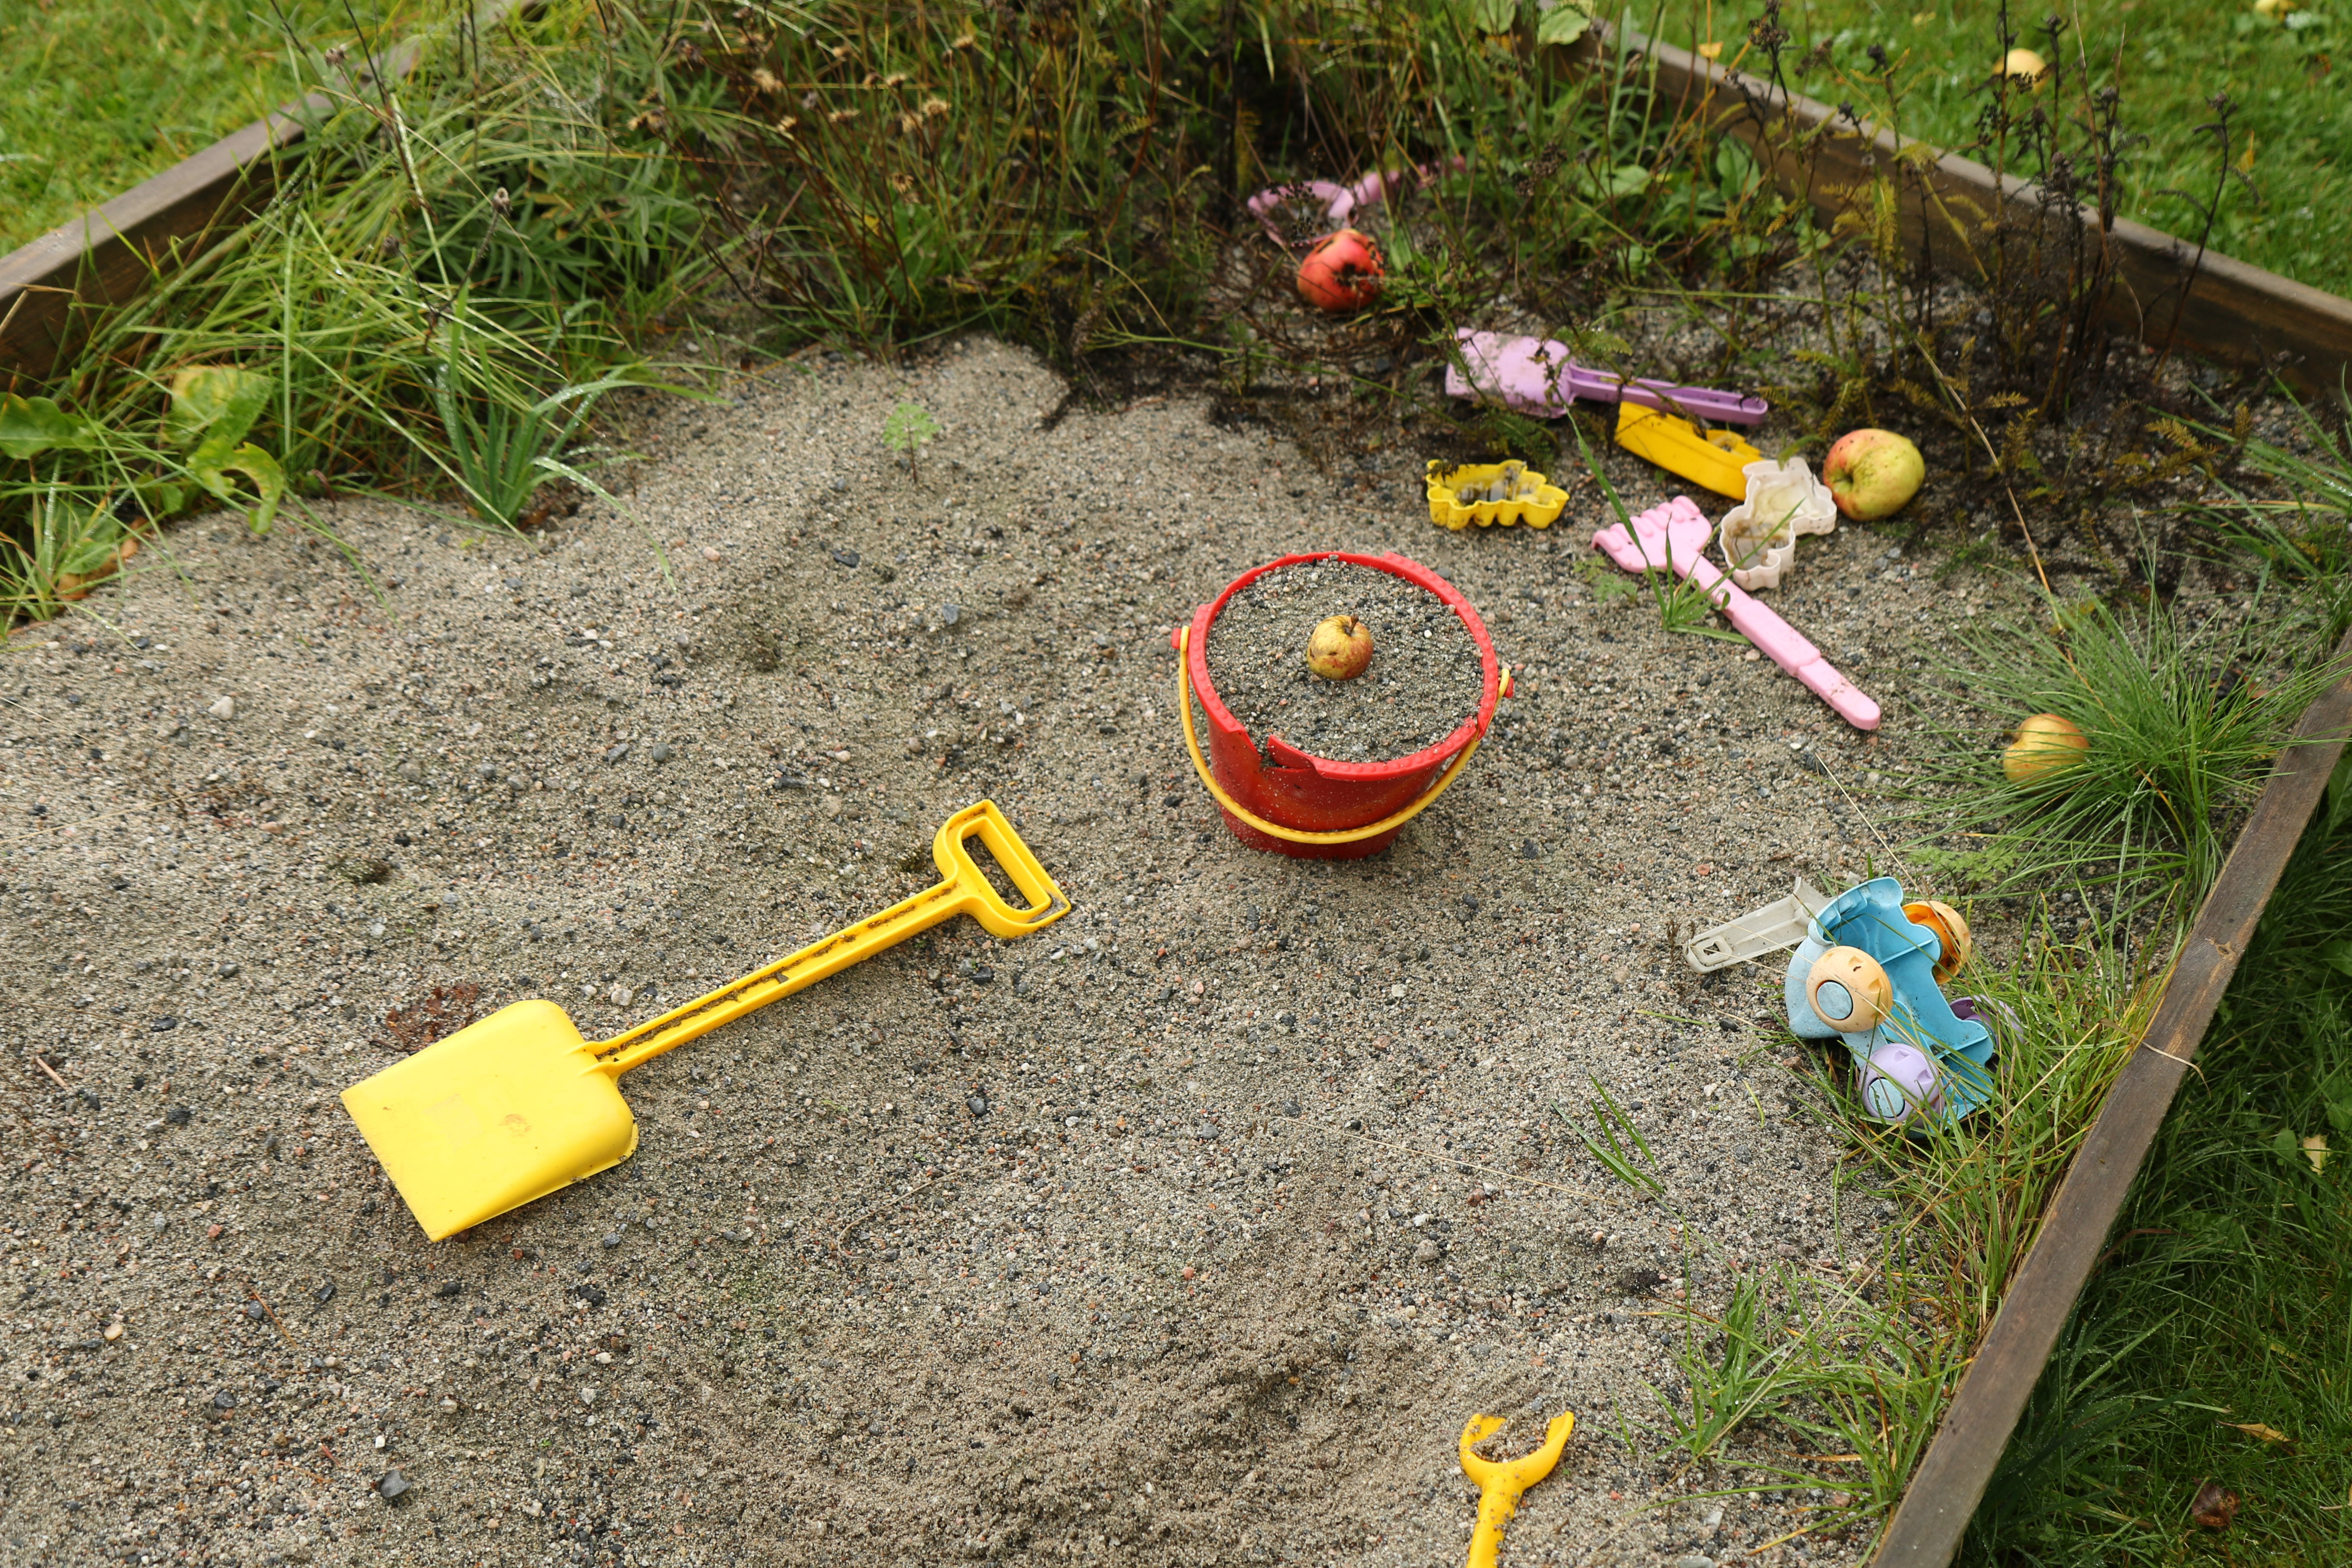
\includegraphics[scale=0.05]{sandbox}
\end{figure}

\end{frame}

sandbox: \verb|https://upload.wikimedia.org/wikipedia/commons/a/a1/Sandkasse_sand_box_Norway.jpg|

\begin{itemize}
\item Developer mode
\item Sandbox
\end{itemize}



\begin{frame}[fragile]
\frametitle{Privacy laws}

\begin{figure}
\includegraphics[scale=0.3]{screen}
\end{figure}

\end{frame}


\begin{itemize}
\item Privacy policy
\item Clear
\item Immutable
\end{itemize}


\begin{frame}[fragile]
\frametitle{Security laws}


\begin{figure}
\includegraphics{security}
\end{figure}

\end{frame}


\begin{itemize}
\item Reasonable care to avoid breaches
\item Breaches must be reported
\item Delay in reporting must be signed off by law enforcement
\end{itemize}

\begin{frame}[fragile]
\frametitle{Fairness in competition laws}


\begin{figure}
\includegraphics[scale=0.1]{scale}
\end{figure}

\end{frame}


\begin{itemize}
\item All devices must allowed all application stores
\item All web services have APIs
\item Local application data format documented
\item Only barrier to API/data access is user consent
\end{itemize}

\begin{frame}[fragile]
\frametitle{Code of Ethics}

\begin{figure}
\includegraphics{fat}
\end{figure}

\end{frame}


\begin{frame}[fragile]
\frametitle{Whistelblowing}

Violations of law must be reported

\end{frame}

\begin{frame}[fragile]
\frametitle{Responsibility to principal}

Except for violations of law,
responsibility is to the development studio.

\end{frame}

\begin{frame}[fragile]
\frametitle{Commitment to competence}

Know your limits

\end{frame}

\begin{frame}[fragile]
\frametitle{Process documentation}

Document disagreements

\end{frame}

\begin{frame}[fragile]
\frametitle{Discrimination and harassment}

Beyond employment law

\end{frame}

\begin{frame}[fragile]
\frametitle{21st century: Incidents}

\begin{itemize}
\item Cambridge analytica
\item Zoom
\item Uber
\end{itemize}

\end{frame}

\begin{frame}[fragile]
\frametitle{If Not Now, When?}

Can we change the timeline?

\end{frame}


Picture credits:

\begin{itemize}
\item Picture of match: \url{https://commons.wikimedia.org/wiki/File:Streichholz.JPG}
\item Picture of fire: \url{https://commons.wikimedia.org/wiki/File:San_Francisco_Fire_Sacramento_Street_1906-04-18.jpg}
\item Picture of lock: \url{https://commons.wikimedia.org/wiki/Category:Padlocks#/media/File:Candados_2012.JPG}
\item Picture of scale: \url{https://commons.wikimedia.org/wiki/Category:Weighing_scales#/media/File:Vaga_MNT.jpg}
\item Picture of screen: \url{https://www.flickr.com/photos/garyjwood/275644014/in/photolist-qmKn1-qmKBr-oYwMG-7UWHnT-EyyT4M-qmL3a-cjf8xs-5wx88t-caR8tq-7QR7pg-6BzSc1-7U9YpL-5v4D74-6C7S53-5i8ZvA-61pcSS-5xP7Hs-5i8ZAA-caR8nd-5hygTA-5htVfK-cjhDRh-5hJXrd-au2jhs-9jX3Pw-7JaQvb-5m5PjW-5i4DBD-5m5PwE-6DPVqE-cttiCW-g5fH57-5wBrCN-6jS7DQ-ctw4mE-5hJXtC-5m5Pph-5hPBJY-6ovsi7-613SBd-6jNe5t-5m5Ptf-5iX6HH-5xRoUn-5i4DMz-5m5Prw-9nXhNt-5m1xre-caR8rh-5htVjc}
\item Picture of red tape: \url{https://commons.wikimedia.org/wiki/File:Redtape1.JPG}
\end{itemize}

\end{document}
